% ||||||||||||||||||||||||||||||||||||||||||||||
% Capitulo de Resultados Preliminares
% ||||||||||||||||||||||||||||||||||||||||||||||

\chapter{Resultados Preliminares}

\begin{figure}[H]
    \caption{Clusters resultantes utilizando a técnica t-SNE com dados sem FFT.}
    \begin{center}
        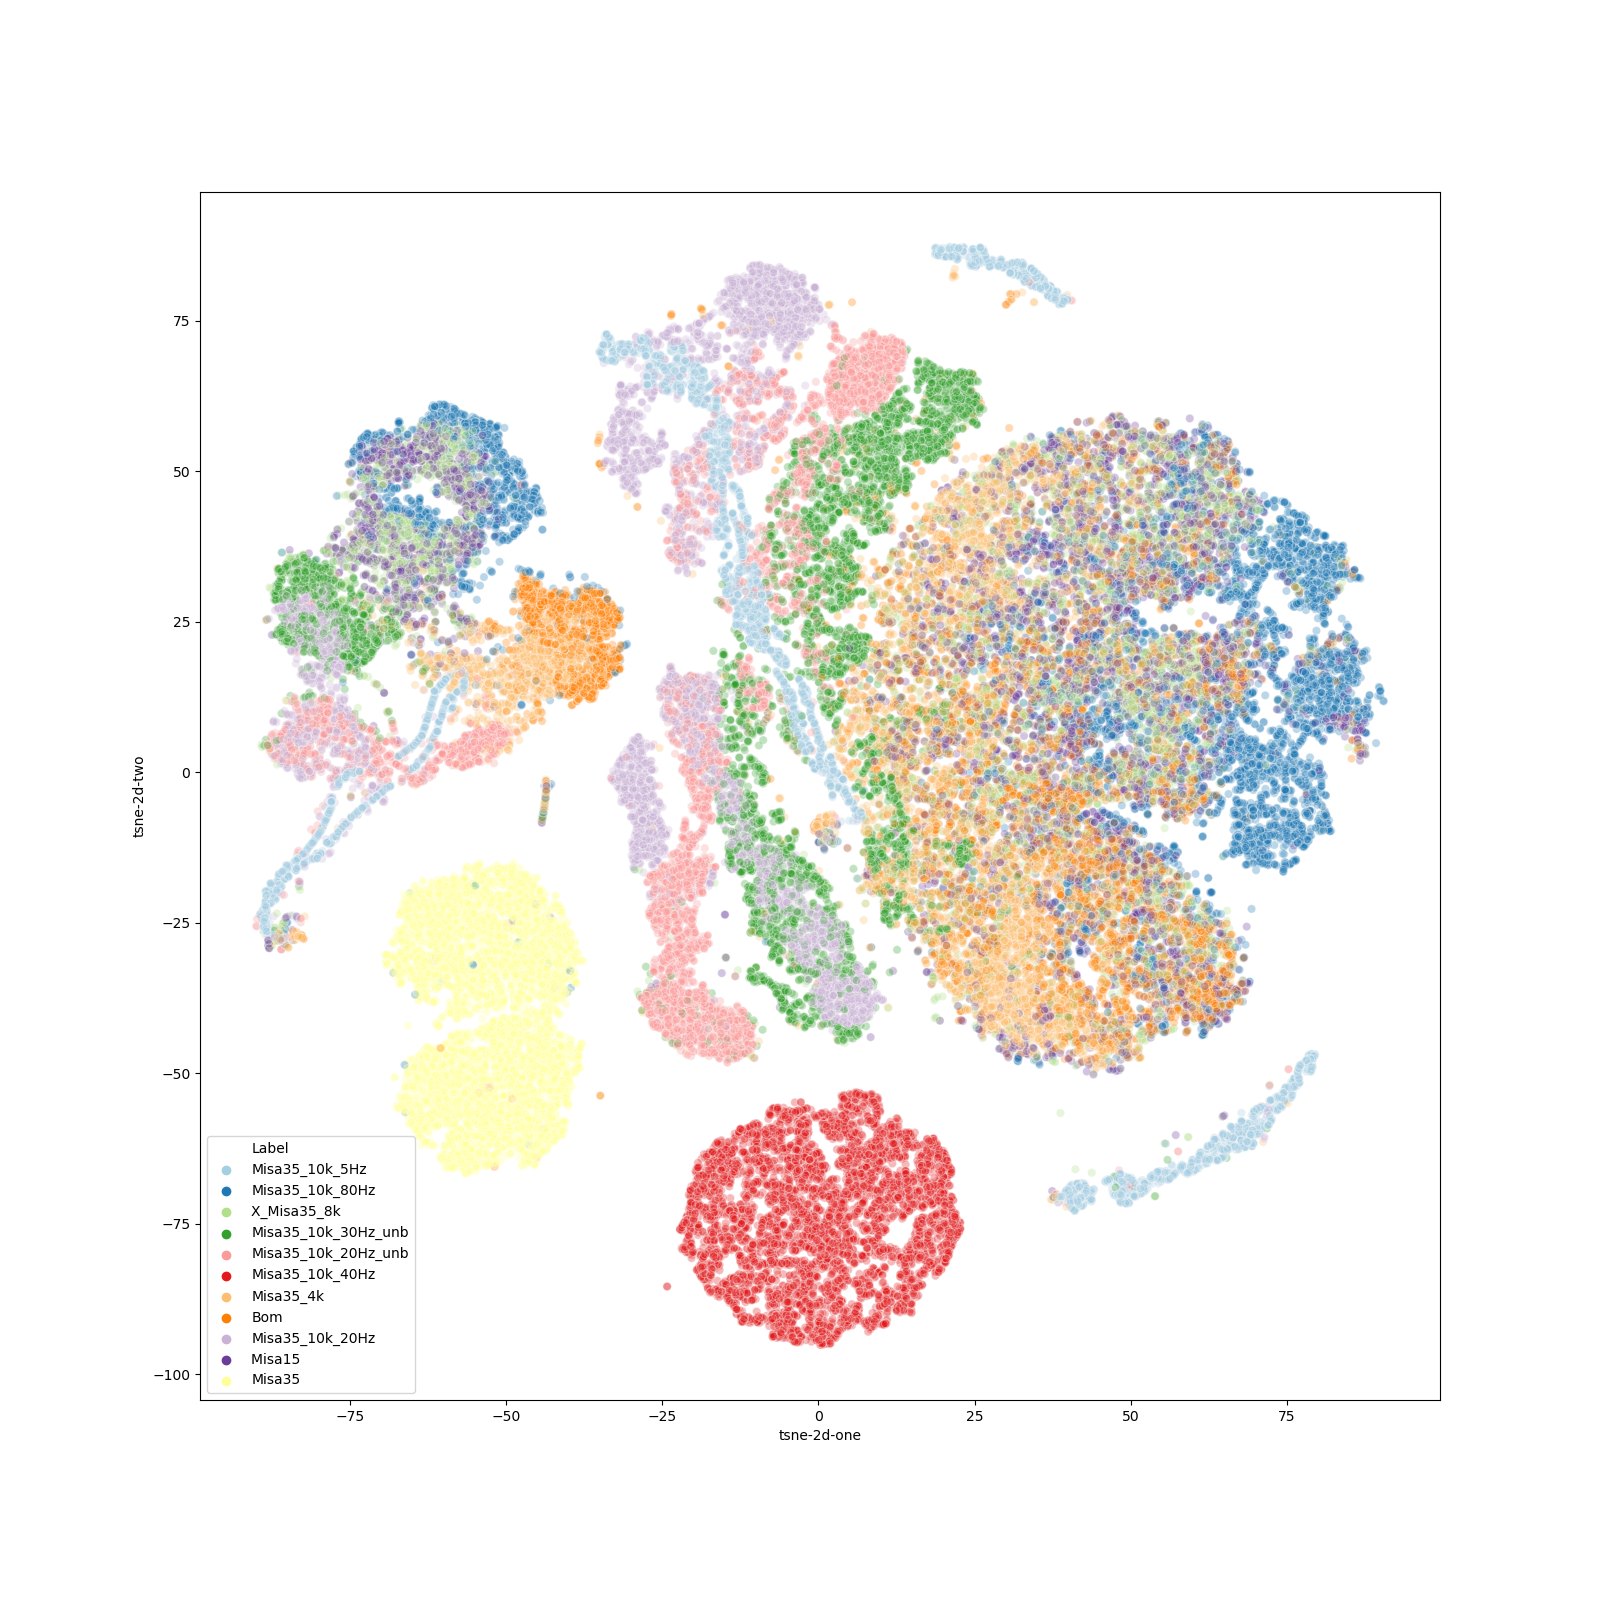
\includegraphics[scale=.25]{resultados/img/t-sne-1.png}
    \end{center}
    \fonte{Elaborado pelo Autor.} 
    \label{fig:}
\end{figure}


\begin{figure}[H]
    \caption{Clusters resultantes utilizando a técnica t-SNE com FFT.}
    \begin{center}
        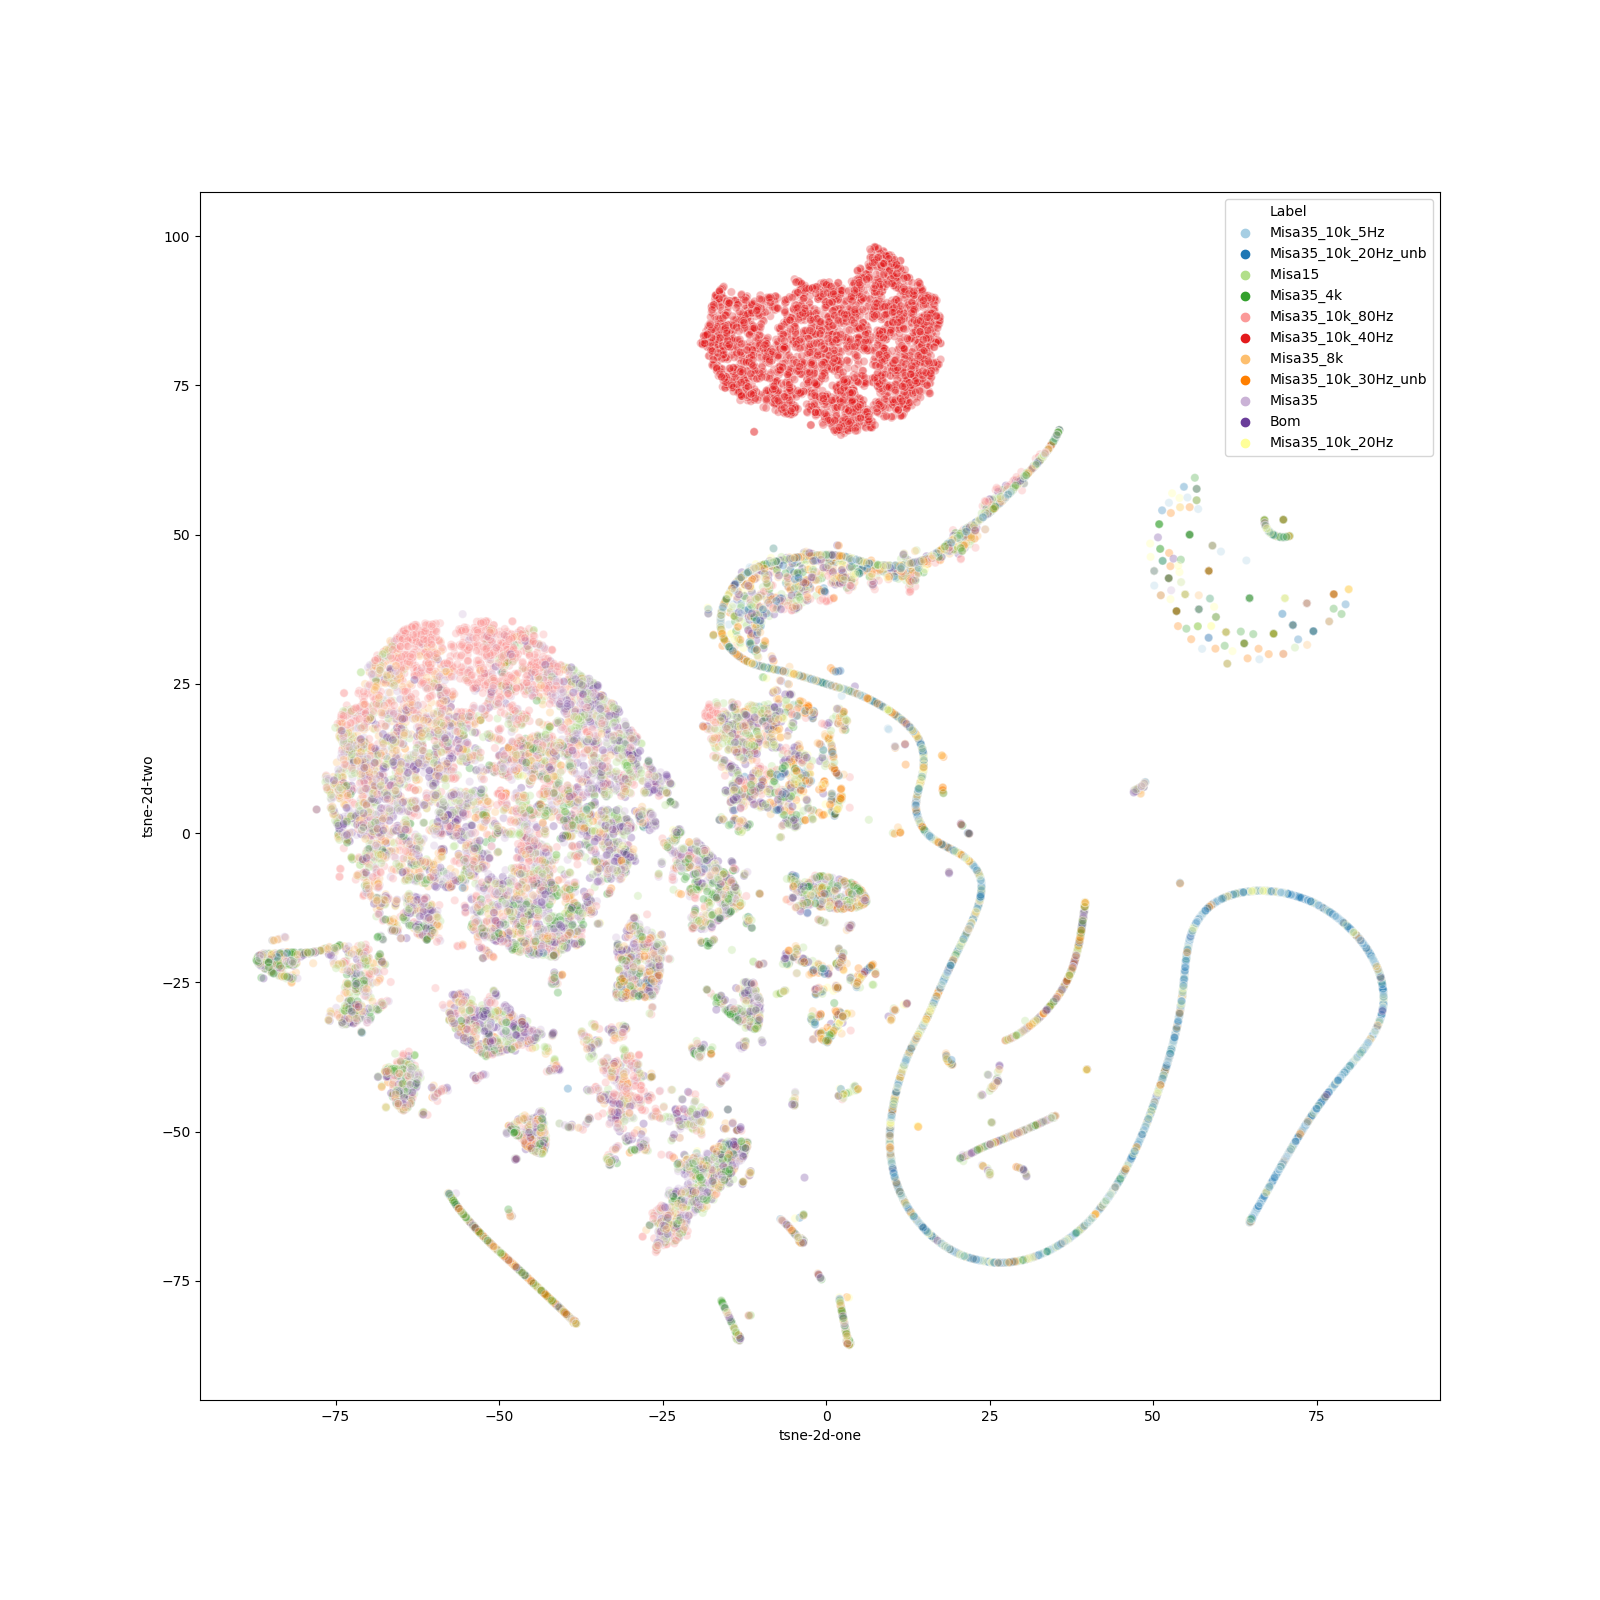
\includegraphics[scale=.25]{resultados/img/fft-t-sne-1.png}
    \end{center}
    \fonte{Elaborado pelo Autor.} 
    \label{fig:}
\end{figure}


\begin{figure}[H]
    \caption{Clusters resultantes utilizando a técnica K-means.}
    \begin{center}
        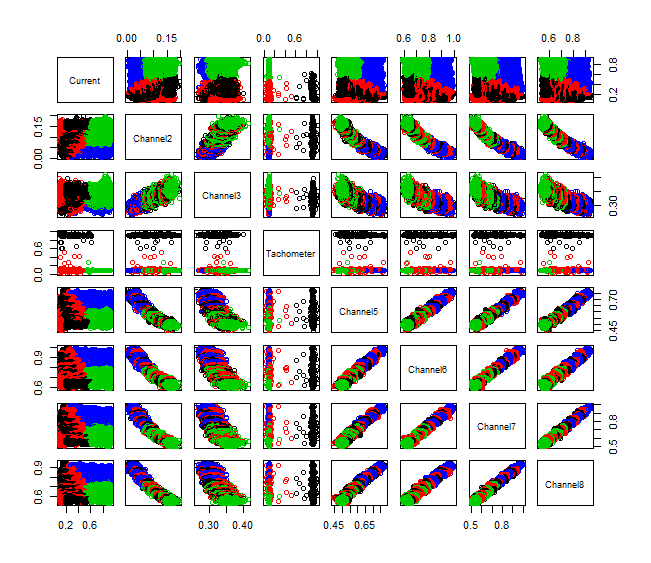
\includegraphics[scale=.65]{resultados/img/kmeans2.png}
    \end{center}
    \fonte{Elaborado pelo Autor.} 
    \label{fig:}
\end{figure}


\begin{figure}[H]
    \caption{Resultados da separação dos dados utilizando a técnica ICA.}
    \begin{center}
        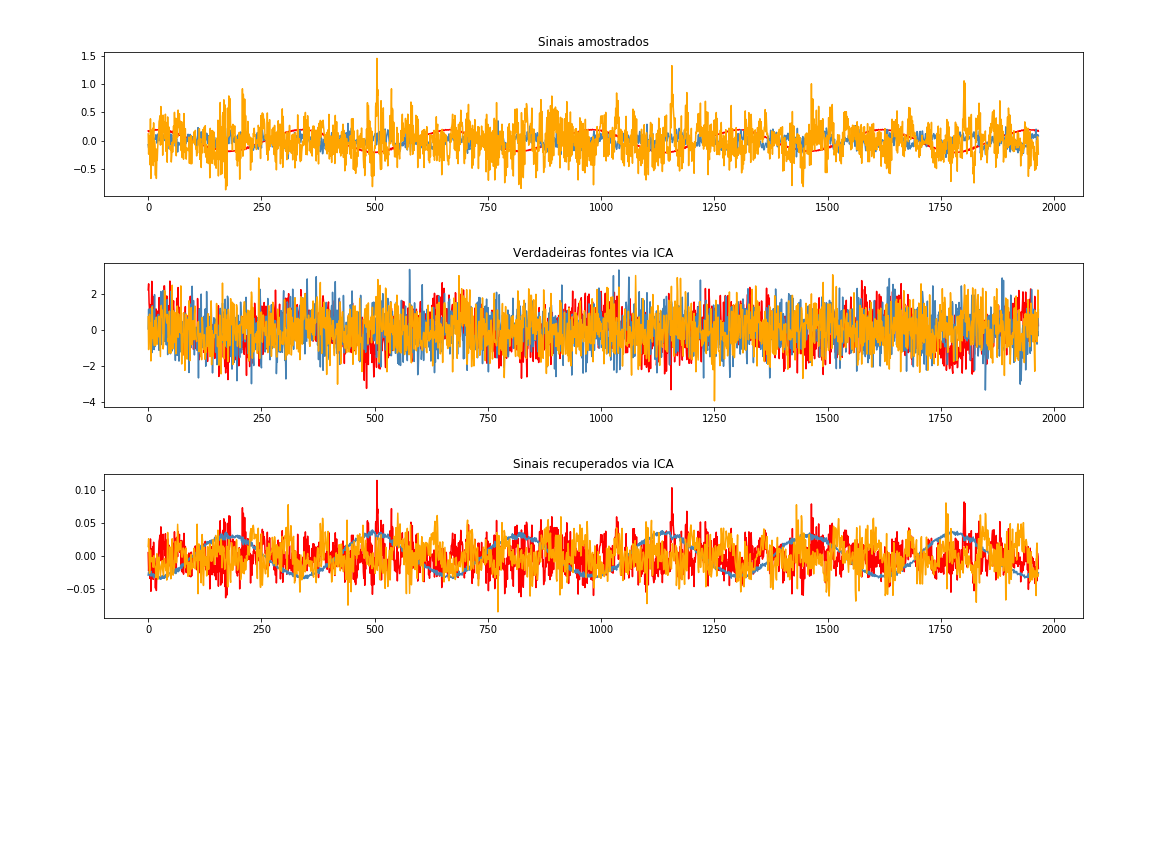
\includegraphics[scale=.4]{resultados/img/ica.png}
    \end{center}
    \fonte{Elaborado pelo Autor.} 
    \label{fig:}
\end{figure}